\subsection{Принцип работы}
Семисегментный светодиодный индикатор — устройство отображения цифровой информации. Это — наиболее простая реализация индикатора, который может отображать арабские цифры. Для отображения букв используются более сложные многосегментные и матричные индикаторы.

\textbf{Семисегментный светодиодный индикатор}, как говорит его название, состоит из семи элементов индикации (сегментов), включающихся и выключающихся по отдельности. Включая их в разных комбинациях, из них можно составить упрощённые изображения арабских цифр.

\begin{figure}[h!]
		\centering
		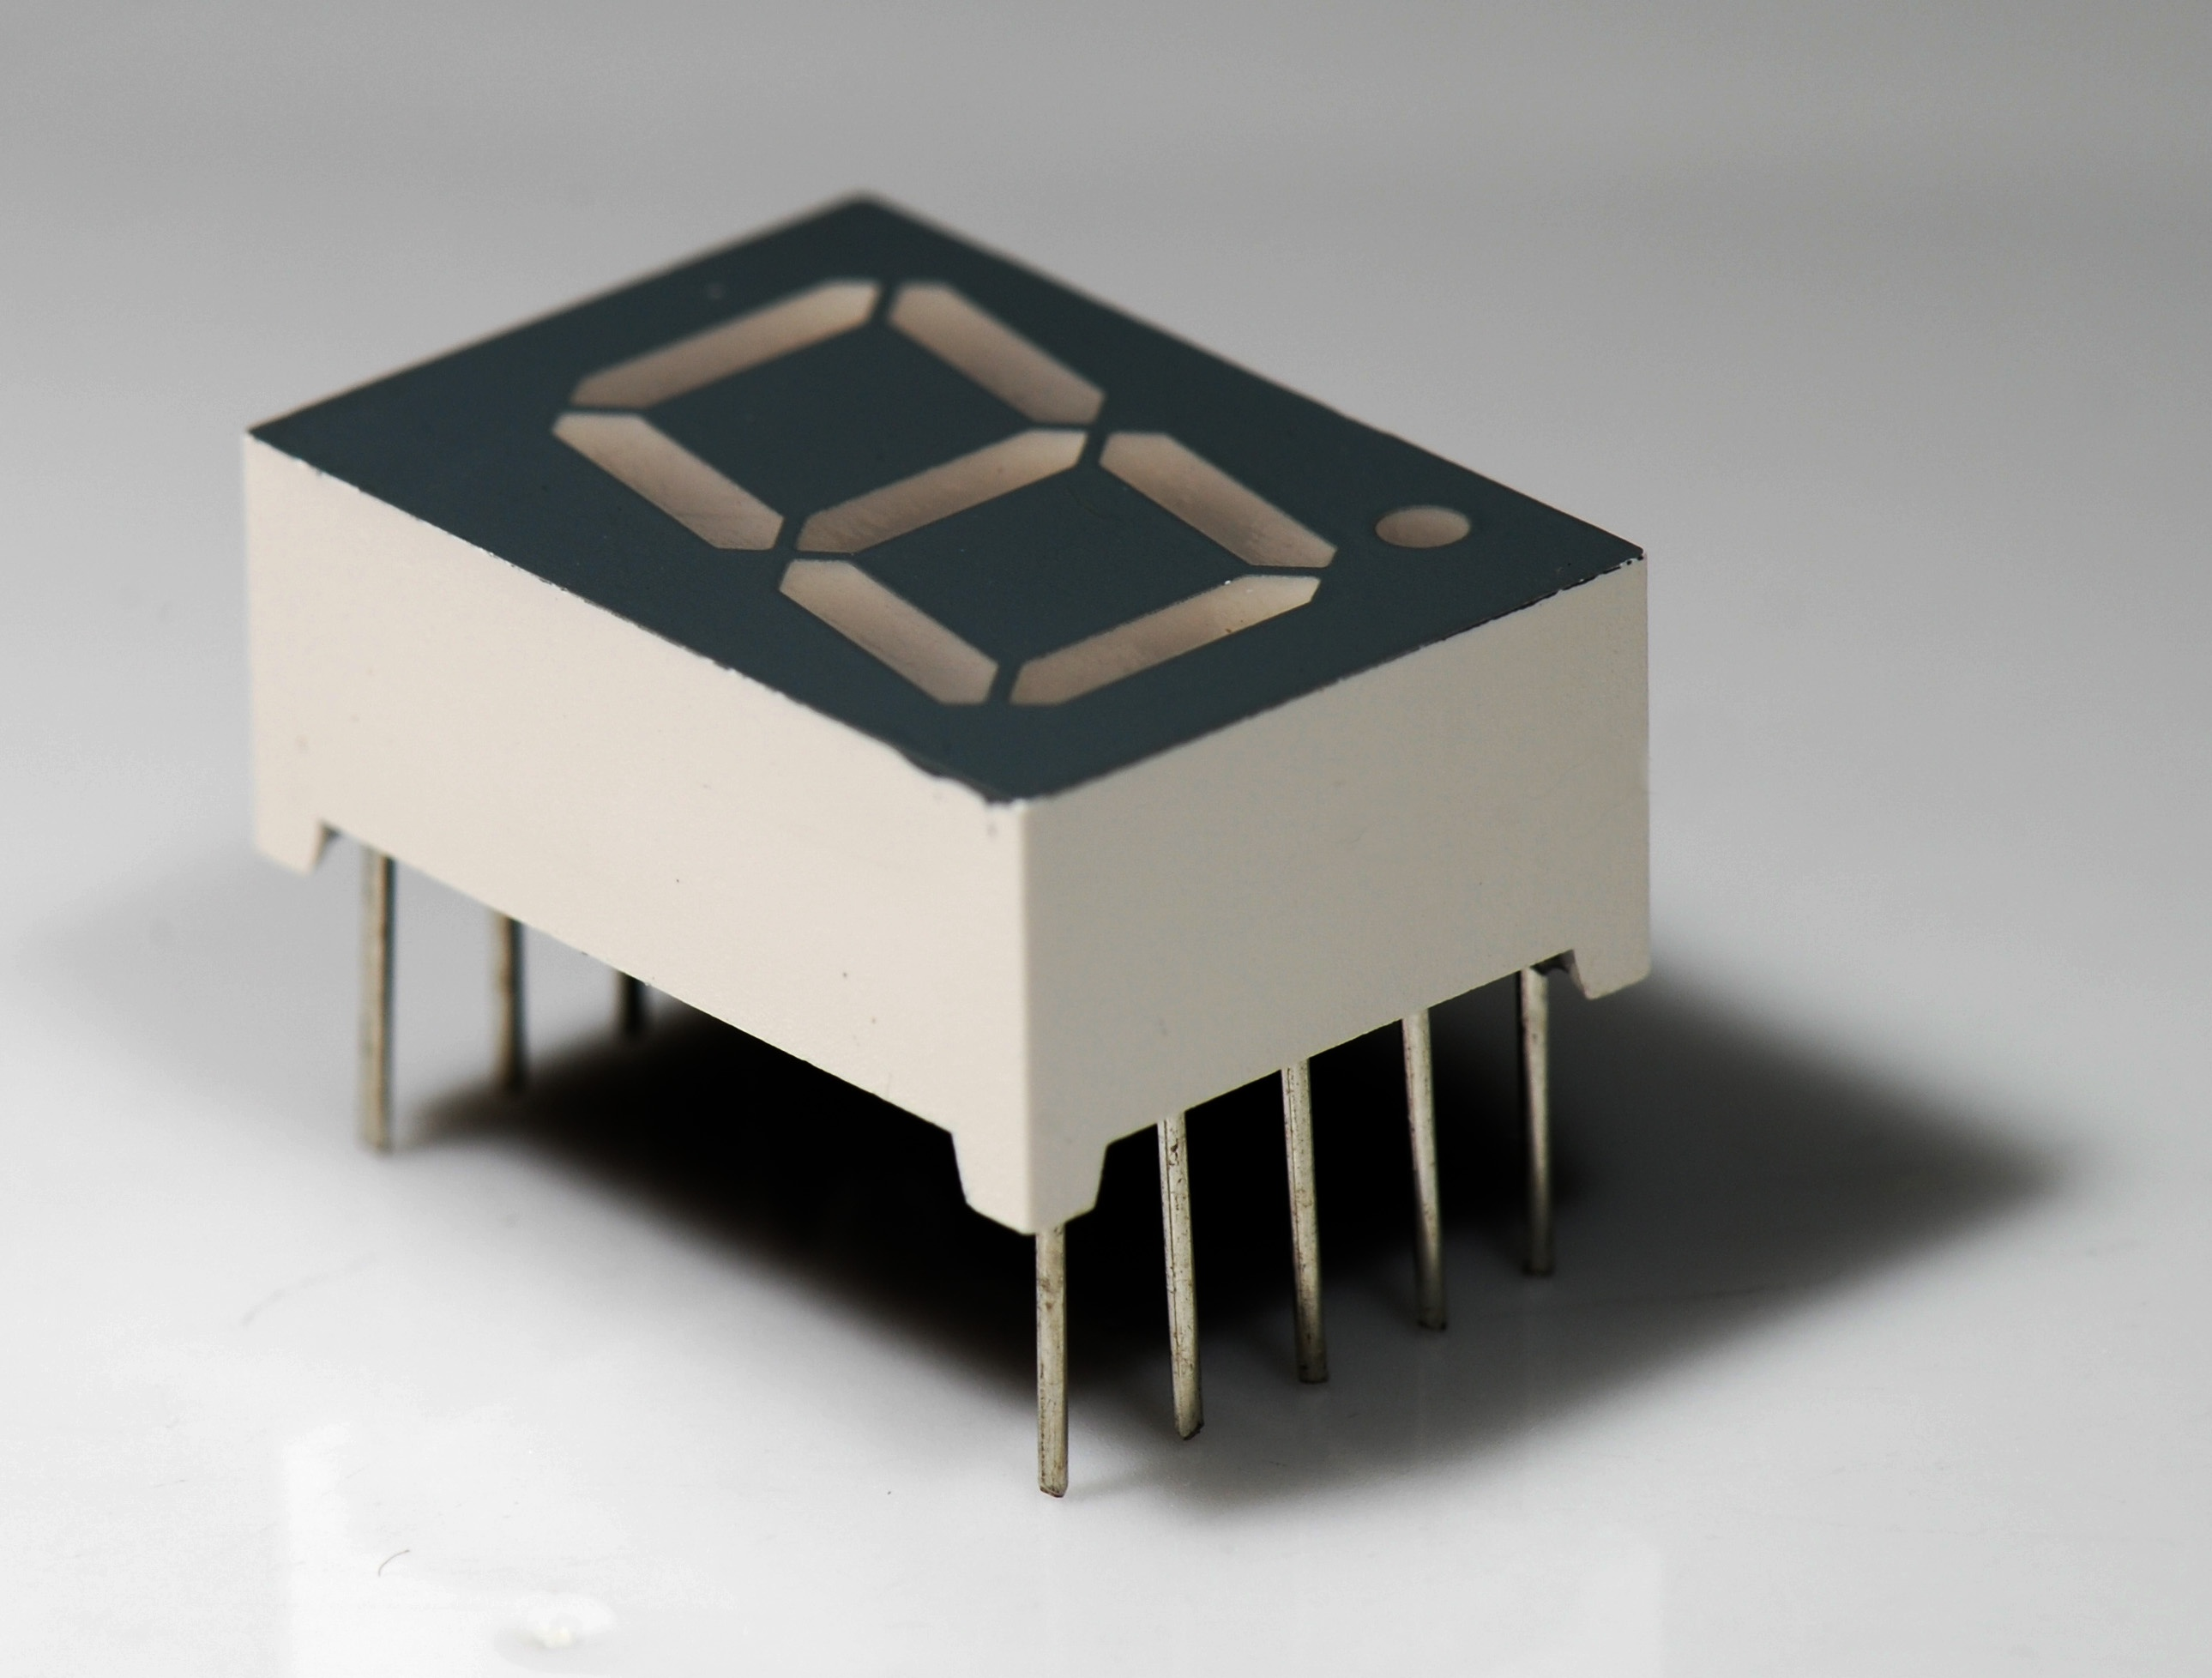
\includegraphics[width=0.8\linewidth]{pics/seven_segment.png}
		\caption{Фото индикатора}
		\label{ind}
\end{figure}

Сегменты обозначаются буквами от A до G; восьмой сегмент — десятичная точка (decimal point, DP), предназначенная для отображения дробных чисел.

Устройство имеет 10 выводов, центральный вывод в каждом ряду это общий анод/катод в зависимости от типа индикатора. Остальные выводы подключаются непосредственно к каждому из сегментов a,b,c,d,e,f,g,dp.


\begin{figure}[h!]
		\centering
		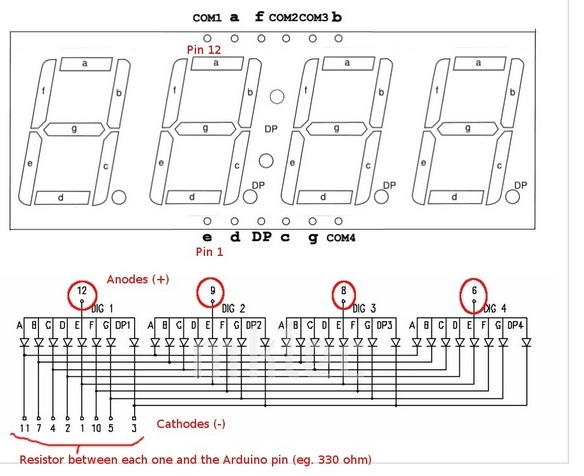
\includegraphics[width=0.8\linewidth]{pics/sem_segmnt_.png}
		\caption{Описание устройства}
		\label{ind}
\end{figure}

При подключении индикатора к микроконтроллеру чтем, что на каждый сегмент необходимо последовательно подключить резистор номиналом $200-300 \: Om$.


